\documentclass[tikz,border=10pt]{standalone}
\usepackage{amsmath}
\usepackage{tikz}
\usetikzlibrary{arrows.meta, positioning, calc, shapes.geometric}

\begin{document}
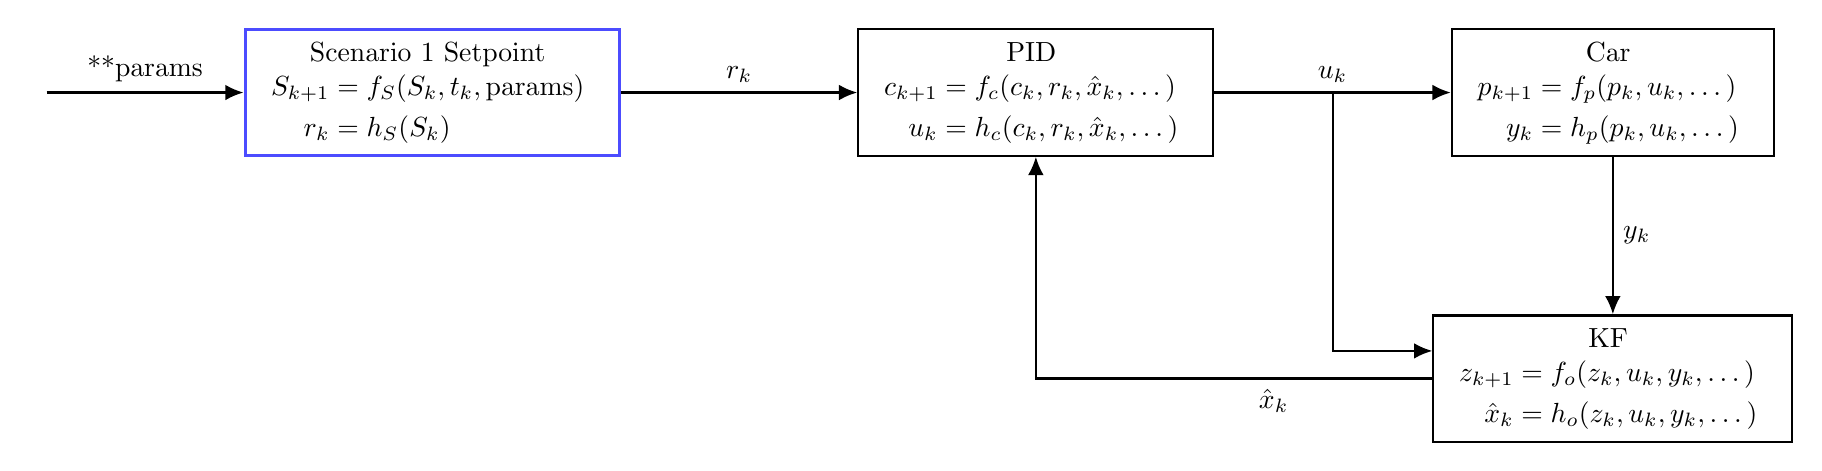
\begin{tikzpicture}[
  block/.style = {draw, thick, minimum height=3em, minimum width=6em, align=center},
  blueblock/.style = {draw=blue!70, very thick, minimum height=3em, minimum width=6em, align=center},
  arrow/.style = {thick, -{Latex[width=2mm]}},
  node distance=2.5cm and 2.5cm
]

  % ======================================================
  % Scenario 1 Setpoint (blue block)
  % ======================================================
  \node[blueblock] (setpoint) {
    \begin{tabular}{c}
      Scenario 1 Setpoint \\
      $\begin{aligned}
        S_{k+1} &= f_S(S_k, t_k, \mathrm{params}) \\
        r_k &= h_S(S_k)
      \end{aligned}$
    \end{tabular}
  };

  % PID Controller (to the right)
  \node[block, right=3.0cm of setpoint] (controller) {
    \begin{tabular}{c}
            PID\\
      $\begin{aligned}
      c_{k+1} &= f_c(c_k, r_k, \hat{x}_k, \dots) \\
      u_k &= h_c(c_k, r_k, \hat{x}_k, \dots)
       \end{aligned}$      
    \end{tabular}
  };

  % Plant
  \node[block, right=3.0cm of controller] (system) {
    \begin{tabular}{c}
      Car\\      
      $\begin{aligned}
      p_{k+1} &= f_p(p_k, u_k, \dots) \\
      y_k &= h_p(p_k, u_k, \dots)
       \end{aligned}$                  
    \end{tabular}
  };

  % Observer (KF)
  \node[block, below=2cm of system] (observer) {
    \begin{tabular}{c}
      KF\\      
    $\begin{aligned}
      z_{k+1} &= f_o(z_k, u_k, y_k, \dots) \\
      \hat{x}_{k} &= h_o(z_k, u_k, y_k, \dots)
       \end{aligned}$            
    \end{tabular}
  };

  % params / b_k input to Scenario 1 Setpoint
  \node[left=2.5cm of setpoint] (params) {};
  \draw[arrow] (params.east) -- node[above] {**params} (setpoint.west);

  % r -> PID
  \draw[arrow] (setpoint.east) -- node[above] {$r_k$} (controller.west);

  % controller -> plant
  \draw[arrow] (controller.east) -- node[above] {$u_k$} (system.west);

  % u branch to observer (split)
  \coordinate (usplit) at ($(controller.east)!0.5!(system.west)$);
  \coordinate[above=1em of observer.west] (observer_uin);
  \draw[arrow] (usplit) |- (observer_uin) node[pos=0.25, right] {};

  % y_p -> observer
  \draw[arrow] (system.south) -- node[right] {$y_k$} (observer.north);

  % observer -> controller (\hat{x}_k feedback)
  \coordinate (controller_yoin) at ($(controller.south)!0.5!(controller.south -| observer.north)$);
  \draw[arrow] (observer.west) -| node[pos=0.2, below] {$\hat{x}_k$} (controller.south);

\end{tikzpicture}
\end{document}
